\paragraph{QuizziPedia::Front-End::Controllers::SignUpController}
\begin{figure} [ht]
	\centering
	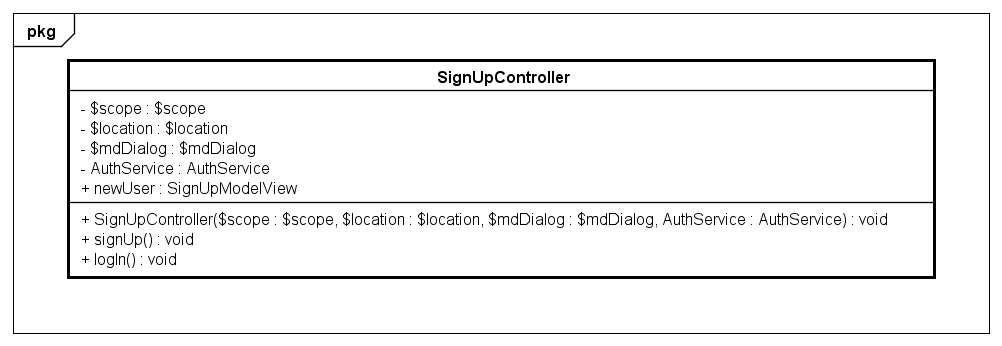
\includegraphics[scale=0.80]{UML/Classi/Front-End/QuizziPedia_Front-end_Controller_SignUpController.png}
	\caption{QuizziPedia::Front-End::Controllers::SignUpController}
\end{figure} \FloatBarrier
\begin{itemize}
	\item \textbf{Descrizione}: questa classe permette di gestire la registrazione di un utente al sistema;
	\item \textbf{Utilizzo}: fornisce le funzionalità di registrazione di un utente al sistema;
	\item \textbf{Relazione con altre classi}:
	\begin{itemize}
		\item \textit{IN} \texttt{SignUpModelView}: classe di tipo modelview la cui istanzazione è contenuta all'interno della variabile di ambiente \$scope di \textit{Angular.js\ped{G}}. All'interno di essa sono presenti le variabili e i metodi necessari per il \textit{Two-Way Data-Binding\ped{G}} tra la view \texttt{SignUpView} e il controller \texttt{SignUpController};
		\item \textit{IN} \texttt{AuthService}: questa classe permette di gestire la registrazione e l'autenticazione di un utente;
	\end{itemize}
	\item \textbf{Attributi}:
	\begin{itemize}
		\item \texttt{-} \texttt{\$scope: \$scope} \\
		Campo dati contenente un riferimento all’oggetto \$scope creato da \textit{Angular\ped{G}}. Viene utilizzato come mezzo di comunicazione tra il controller e la view. Contiene gli oggetti che definiscono il viewmodel e il model dell’applicazione;
		\item \texttt{-} \texttt{\$location: \$location} \\
		Campo dati contenente un riferimento al servizio creato da \textit{Angular\ped{G}} che permette di accedere alla barra degli indirizzi del \textit{browser\ped{G}}, i cambiamenti all’URL nella barra degli indirizzi si riflettono in questo oggetto e viceversa;
		\item \texttt{-} \texttt{\$mdDialog: \$mdDialog} \\
		Campo dati contenente un riferimento al servizio della libreria \textit{Material for Angular\ped{G}} che permette di creare delle componenti a popup;
		\item \texttt{-} \texttt{AuthService: AuthService} \\
		Campo dati contenente un riferimento al servizio che si occupa della gestione delle informazioni legate all’autenticazione. Viene utilizzato il metodo \texttt{signUp} di \$texttt{AuthService} a cui viene passato come parametro un oggetto di tipo \texttt{SignUpModelView};
		\item \texttt{+} \texttt{newUser: SignUpModelView} \\
		Oggetto di tipo \texttt{SignUpModelView}. All'interno di esso sono presenti le variabili e i metodi necessari per il \textit{Two-Way Data-Binding\ped{G}} tra la view \texttt{SignUpView} e il controller \texttt{SignUpController};
	\end{itemize}
	\item \textbf{Metodi}:
	\begin{itemize}
		\item \texttt{+} \texttt{SignUpController(\$scope: \$scope, \$location: \$location, \$mdDialog: \$mdDialog, AuthService: AuthService)} \\
		Metodo costruttore della classe: \\
		\textbf{Parametri}:
		\begin{itemize}
			\item \texttt{\$scope: \$scope} \\
			Parametro contenente un riferimento all’oggetto \$scope creato da \textit{Angular\ped{G}}. Viene utilizzato come mezzo di comunicazione tra il controller e la view. Contiene gli oggetti che definiscono il viewmodel e il model dell’applicazione;
			\item \texttt{\$location: \$location} \\
			Parametro contenente un riferimento al servizio creato da \textit{Angular\ped{G}} che permette di accedere alla barra degli indirizzi del \textit{browser\ped{G}}, i cambiamenti all’URL nella barra degli indirizzi si riflettono in questo oggetto e viceversa;
			\item \texttt{\$mdDialog: \$mdDialog} \\
			Parametro contenente un riferimento al servizio della libreria \textit{Material for Angular\ped{G}} che permette di creare delle componenti a popup;
			\item \texttt{AuthService: AuthService} \\
			Campo dati contenente un riferimento al servizio che si occupa della gestione delle informazioni legate all’autenticazione. Viene utilizzato il metodo \texttt{logIn} di \$texttt{AuthService} a cui vengono passati i parametri \texttt{username} e \texttt{password};
		\end{itemize}
		\item \texttt{+} \texttt{signUp(user: Object): void} \\
		Metodo che richiama il metodo \texttt{signup} del service \texttt{AuthService} passandogli un oggetto di tipo \texttt{SignUpModelView}. Nel caso di buona riuscita dell'operazione viene mostrato un messaggio di successo. Con l'azione di click sul bottone presentato dal messaggio di successo è possibile effettuare il redirect alla pagina di login dell'applicazione. Nel caso in cui invece avvenga un errore, viene mostrato a video il messaggio di errore;
		\item \texttt{+} \texttt{logIn(): void} \\
		Metodo che gestisce l’evento click sul pulsante di login. Effettua il redirect alla pagina di login;
	
	\end{itemize}
\end{itemize}

